\begin{tikzpicture}
	\pgfmathsetlengthmacro{\height}{5.1cm}
	
	\pgfmathsetlengthmacro{\machineheight}{\height}
	\pgfmathsetlengthmacro{\manheight}{\height * (177.8cm/192.2cm)}
	
	\node (machine)
	      [inner sep=0]
	      {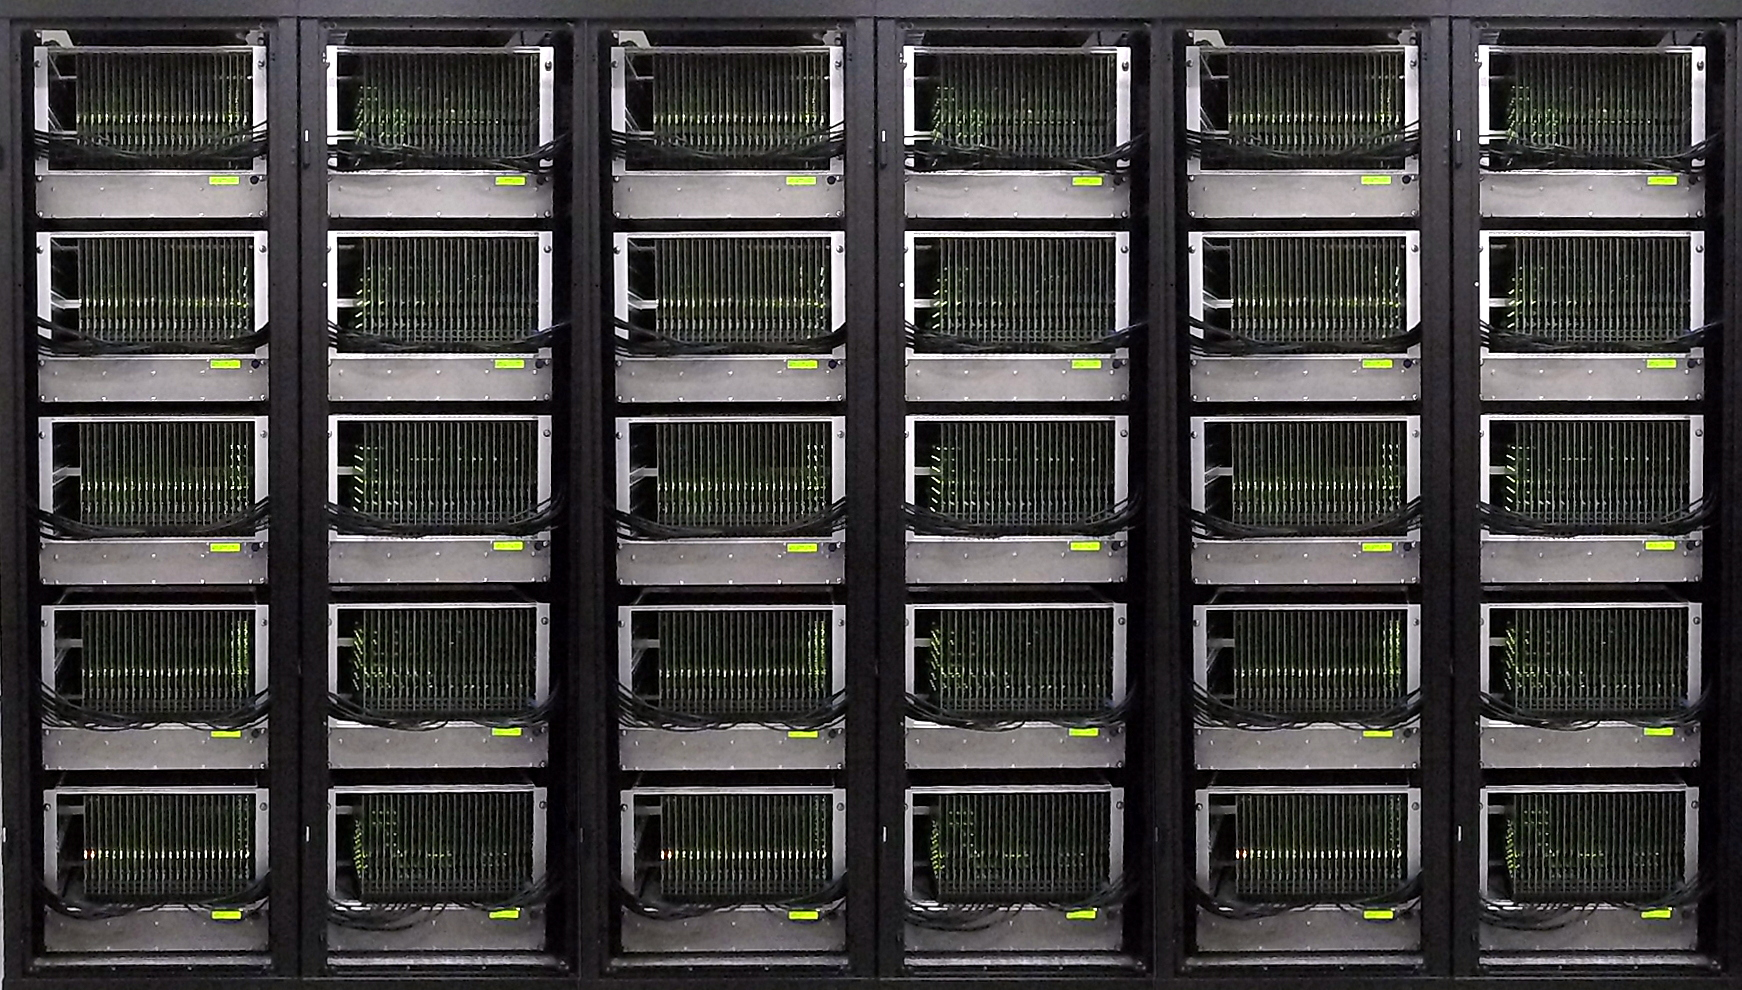
\includegraphics[height=\machineheight]{figures/six_cabinets.jpg}};
	
	\node (person)
	      [ right=2mm of machine.south east
	      , inner sep=0
	      , anchor=south west
	      ]
	      {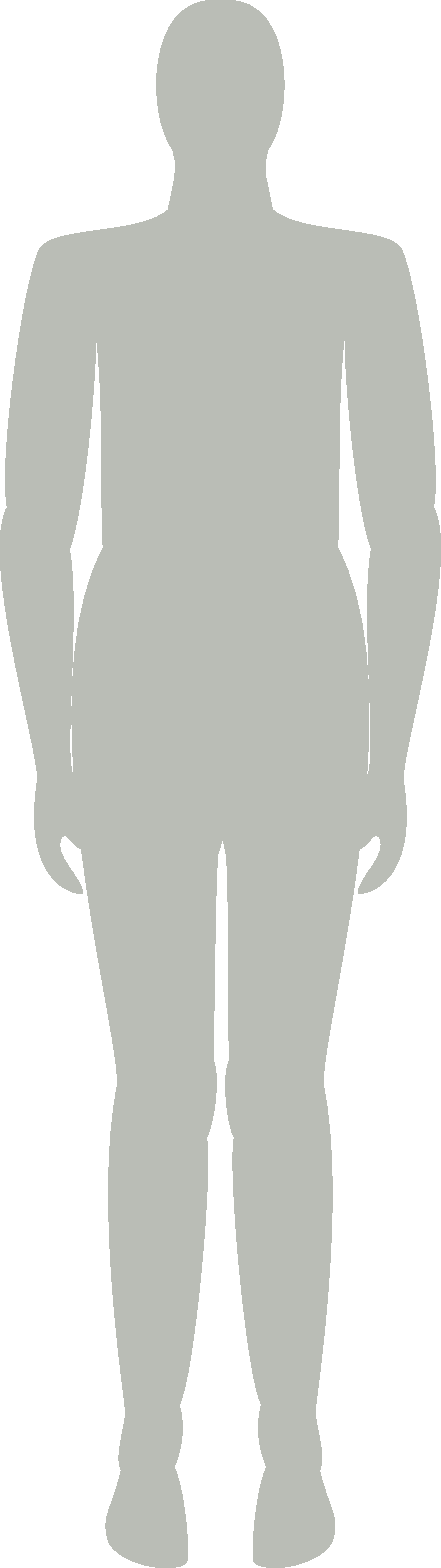
\includegraphics[height=\manheight]{figures/person.pdf}};
	
	\draw [decorate
	      , decoration={ brace
	                   , amplitude=0.3em
	                   , raise=0.2em
	                   }
	      ]
	      ($(machine.north west)!0.00!(machine.north east)$)
	   -- node [anchor=south,yshift=0.5em,align=center]
	           {19\inch{} cabinet}
	      ($(machine.north west)!0.166!(machine.north east)$);
	
	\draw [decorate
	      , decoration={ brace
	                   , amplitude=0.3em
	                   , raise=0.2em
	                   }
	      ]
	      ($(machine.south west)!0.83!(machine.north west)$)
	   -- node [anchor=east,xshift=-0.5em,align=right]
	           {Frame\\\footnotesize{}(5 per cabinet)}
	      ($(machine.south west)!0.96!(machine.north west)$);
	
	\coordinate (board) at ([xshift=1.0em]$(machine.south west)!0.12!(machine.north west)$);
	\draw [rounded corners]
	      (machine.west |- board)
	   -| ++(-2.0em, 0.50em)
	      node [anchor=south, align=right,xshift=-1.6em]
	           {SpiNNaker\\board\\\footnotesize{}(24 per frame)}
	      ;
	\draw [<-,white] (board) -- (machine.west |- board);

\end{tikzpicture}

